\subsection{Purpose} 
Agriculture has a key role in India's economy and covid-19 pandemic has highlighted the need of building a resilient food system.
This need is increased by the problems due to climate change that will impact everything from productivity to 
livelihoods across food and farm systems and is predicted to result in a 4\%-26\% loss in net farm income towards the end of the century.
In addition, according to Harvard Business Review, food demand is expected to increase between 59\% to 98\% by 2050.\\
For this reason policy makers, citizens, agronomists, and farmers should share data and information to achieve better results. 
\\\\
Telangana region is an extended and populous state of India, whose economy is mainly driven by agriculture. 
To address the described above problem, Telangana's government want to design, 
develop and demonstrate anticipatory governance models for food system using digital 
public goods and community-centric approaches to strengthen data-driven policy-making in the state.
\\\\
The application aims to enable the acquisition, communication and combination of data provided by Telangana policymakers, 
farmers and agronomists as:
\begin{itemize}
    \item meteorological forecasts
    \item farmers' production
    \item amount of used water
    \item soil humidity
    \item agronomists' report
\end{itemize}
\bigskip
The product will allow policymakers to identify farmers who are performing well and those who are performing badly. 
As the first ones will receive special incentives and will be asked to provide useful best practices to others. 
Furthermore, the application will provide information regarding the results of the farmers who received help.
\\\\
The product needs to provide farmers the ability to visualize data relevant to them based on their location and type of production. 
Farmers should be also able to insert in the system data about production and any problem they face. 
They should be allowed to send help requests to agronomists and create forum discussion with agronomists or other farmers.
\\\\
The application will allow agronomists to insert the area they are responsible for, receive information about requests for help, 
and answer them. Agronomists need to know data about weather forecasts and the best performing farmers in the area; 
they also need to visualize and update daily plan visits of farms. At the end of each day the agronomist need to confirm the daily
schedule.

\subsection{Scope}
To represent the scope of the project we use the "The World and The Machine" model by M. Jackson. 
It contains the events which cannot be observed by the system ("The World"), 
those strictly related to the system ("The Machine"), and those in common between them. 

\newpage
\begin{figure}[H]
    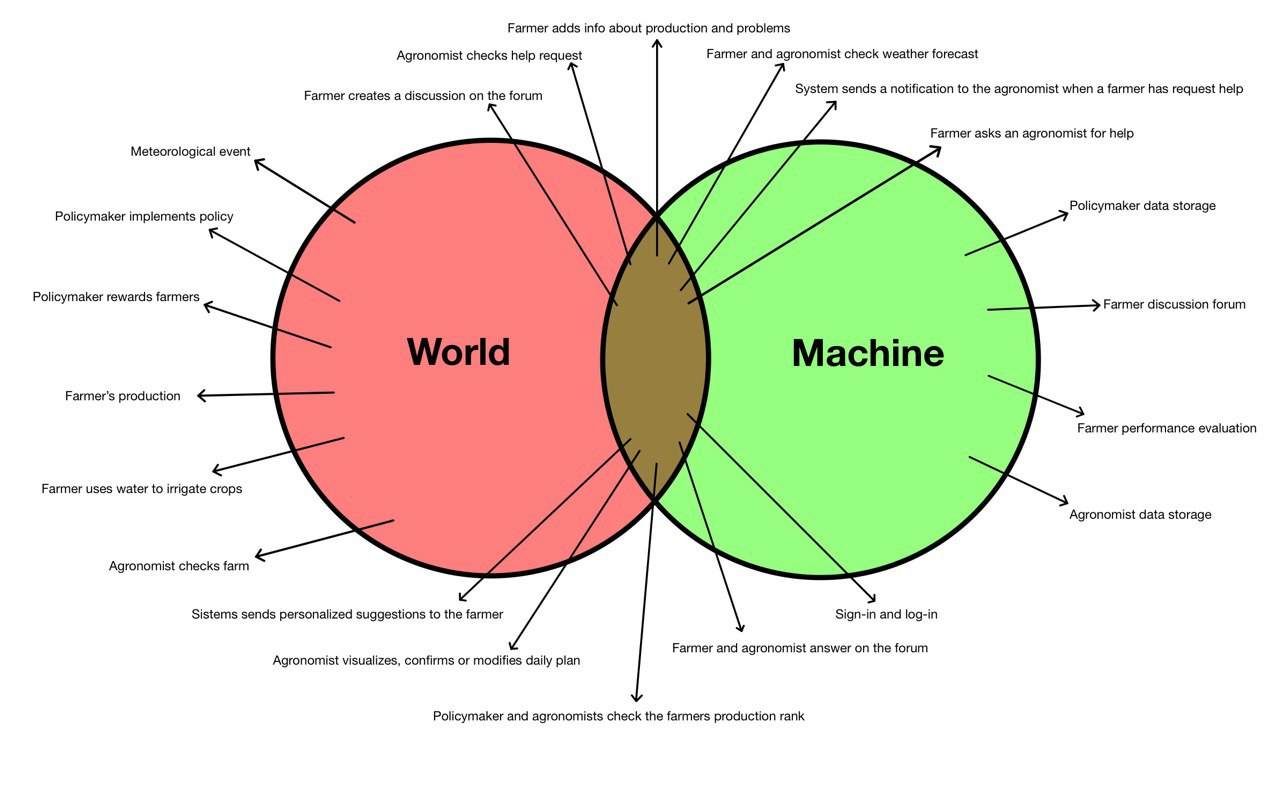
\includegraphics[width=\textwidth,height=\textheight,keepaspectratio]{Images/WorldAndMachine.jpg}
    \caption{The World and the Machine diagram}
    \label{fig:WorldAndMachine}
\end{figure}

\subsubsection{World phenomena}
\begin{itemize}
    \item Meteorological event
    \item Policymaker implements policy
    \item Policymaker rewards farmers
    \item Farmer's production
    \item Farmer uses water to irrigate crops
    \item Agronomist checks farm
\end{itemize}

\subsubsection{Machine phenomena}
\begin{itemize}
    \item Policymaker data storage
    \item Farmer discussion forum
    \item Farmer performance evaluation
    \item Agronomist data storage
\end{itemize}

\subsubsection{Shared phenomena}
\paragraph{Controlled by the World}
\begin{itemize}
    \item Policymaker and agronomist check the farmers production leaderboard
    \item Policymaker sign-in and log-in
    \item Farmer answers discussions on the forum
    \item Farmer sign-in and log-in 
    \item Farmer add information about his production
    \item Farmer add information about a problem he faces
    \item Farmer create a discussion on the forum about a problem
    \item Farmer checks weather forecasts
    \item Farmer asks an agronomist for help
    \item Agronomist sign-in and log-in
    \item Agronomist checks help requests
    \item Agronomist answers help request on the forum
    \item Agronomist answers privately help request
    \item Agronomist checks weather forecasts
    \item Agronomist visualizes daily plan
    \item Agronomist confirms or modifies daily plan
\end{itemize}

\paragraph{Controlled by the Machine}
\begin{itemize}
    \item System sends personalized suggestions to the farmer
    \item System sends a notification to the agronomist when a farmer has requested help
\end{itemize}

\subsubsection{Goals}

\begin{description}
    \item [G1] The app should help and improve farmers' work-related activity
    \item [G2] The app should allow agronomists to oversee and improve farmers work
    \item [G3] The app should allow policymakers to control agriculture performance in Telangana
\end{description}

\subsection{Definitions, Acronyms, Abbreviations}

\subsubsection{Definitions}

\begin{description}
    \item [User] Everyone who is interested in using \emph{DREAM}
    \item [Farmer] Person who owns a farm and needs to be helped using \emph{DREAM}
    \item [Agronomist] Specialized individual who wants to help and monitor farmers through \emph{DREAM}
    \item [Policymaker] Government official who wants to supervise the agricultural sector
    \item [Forum] Section of \emph{DREAM}, accessible for farmers and agronomists, used to discuss farmers' problems
\end{description}

\subsubsection{Acronyms}

\begin{description}
    \item [DREAM] Data-dRiven prEdictive fArMing
    \item [RASD] Requirement Analysis and Specification Document
    \item [HTTPS] Hypertext Transfer Protocol over Secure Socket Layer
    \item [UML] Unified Modeling Language
    \item [MITM] Man-In-The-Middle
\end{description}

\subsubsection{Abbreviations}

\begin{description}
    \item [{[Gn]}] n-th goal.
    \item [{[Dn]}] n-th domain assumption.
    \item [{[Rn]}] n-th functional requirement.
\end{description}

\bigskip
\subsection{Revision history}

\begin{description}
    \item[v. 1.0 - 23/12/2021] Initial release
\end{description} 

\bigskip
\subsection{Reference documents}

\begin{description}
    \item [WeBeeP channel] - Project Assignment
    \item [The World \& The Machine] - M. Jackson, P. Zave 
\end{description}

\bigskip
\subsection{Document structure}

This document is structured in the following five main chapters:

\begin{enumerate}
    \item[\textbf{Chapter 1}] This chapter offers a brief description of the problem and required functionalities. It also
    contains the list of definitions, acronyms and abbreviations that could be found in this document. 

    \item[\textbf{Chapter 2}] The second chapter offers a summary description about the overall organization of the system 
    (through state machine diagrams), the hardware and the software costraints. 
    It also contains a description of all the features, the actors who used them.

    \item[\textbf{Chapter 3}] This section contains mockups interfaces in order to explain those mentioned in Chapter 2.
    It also contains a description of functional requirement through some scenarios, use cases and sequence diagrams. 

    \item[\textbf{Chapter 4}] The fourth chapter is a formal analysis of the model, made through the Alloy, including a graphic representation of it obtained from Alloy Tool.

    \item[\textbf{Chapter 5}] The fifth and last chapter contains the efforts spent by each contributor.
\end{enumerate}
